\subsection{Antlr-Grammatik}\label{subsec:antlr-grammatik}
Da die möglichen Eingaben durch das zuvor beschriebene JSON-Schema bereits verringert wurden, fiel die Wahl der Verarbeitung der YAML-Eingabe auf einen durch Antlr generierten Parser.
Dieser bietet die Möglichkeit, während dem Parsen weitere Aktionen durchzuführen und in dem Fall dieser Anwendung ein Datenmodell aus der Eingabe zu erstellen.
Das Datenmodell wird im folgenden weiterverarbeitet und bietet somit eine Grundlage für die Generierung, auf welche im folgenden Kapitel eingegangen wird.

Wie in Kapitel~\ref{subsubsec:antlr} bereits beschrieben, ist die Grundlage eines Antlr-Parsers die dazugehörige Grammatik, welche nun beleuchtet wird.
Die komplette Grammatik ist im referenzierten fulibWorkflows-Repository im Anhang hinterlegt, in diesem Kapitel werden lediglich Ausschnitte daraus verwendet.
Im Folgenden wird anstatt Zettel zur Beschreibung eines Post-its die englische Übersetzung ``Note'' verwendet, um einen direkten Bezug zu den nachfolgenden Listings herzustellen.

\begin{listing}[!ht]
    \inputminted[firstnumber=5]{antlr-java}{listings/3.1.3/Main.g4}
    \caption{Grammatik für Workflows}
    \label{listing:main-grammar}
\end{listing}

Zuerst wird die grundlegende Struktur einer Datei festgelegt, dies ist durch die drei Regeln in Listing~\ref{listing:main-grammar} dargestellt.
Da eine Datei mehrere Workflows beinhalten kann, ist die oberste Regel in Zeile 5 der Startpunkt des Parsers.
Da als Eingabe eine YAML-Datei ist, heißt die oberste Regel \textit{file} und erfordert mindestens einen~\textit{workflow}.
Ein~\textit{workflow} besteht immer aus einem workflow-Note und beliebig vielen event-Notes, wobei diese immer mit einer Leerzeile von einander getrennt sind.
Die Spezifikation ist aufgrund der YAML-Syntax notwendig.
Ein event-Note ist immer einem von drei Typen zuzuordnen, wobei nach einem Note beliebig viele Leerzeilen folgen können.

\begin{listing}[!ht]
    \inputminted[firstnumber=11]{antlr-java}{listings/3.1.3/Note.g4}
    \caption{Grammatik für Notes}
    \label{listing:note-grammar}
\end{listing}

Die Unterscheidung zwischen normal-/extended-Note, workflow und page erfolgt durch das Schlüsselwort, welches zwischen Bindestrich (\textbf{MINUS}) und Doppelpunkt (\textbf{NAME}) befindet.
Sowohl ein workflow-Note als auch die normal-Notes besitzen lediglich nach dem Doppelpunkt einen Wert, welcher durch \textbf{NAME} gekennzeichnet ist.
Dies ist in Listing~\ref{listing:note-grammar} in Zeile 11 und 13 dargestellt.
Ein extended-Note besitzt neben dem Wert zusätzliche Attribute, welche in einer neuen Zeile beschrieben werden.
Die Anzahl der Attribute ist beliebig, es ist somit erlaubt einen extended-Note ohne weitere Attribute anzugeben.
Die Page ist wie zuvor bereits erwähnt ein Sonderfall, welches sich auch in der Grammatik widerspiegelt.
Dem Schlüsselwort \textit{page} folgt ein gesonderter Doppelpunkt und anschließend eine Liste von neuen Elemente.

\begin{listing}[!ht]
    \inputminted[firstnumber=30]{antlr-java}{listings/3.1.3/Keywords.g4}
    \caption{Schlüsselwörter zum Identifizieren von Notes}
    \label{listing:note-ids}
\end{listing}

Die zuvor erwähnten normal-Notes bestehen wie in Listing~\ref{listing:note-ids} Zeile 30 und 31 dargestellt aus \textit{externalSystem}, \textit{service}, \textit{command}, \textit{policy}, \textit{user} und \textit{problem}.
Diese erhalten lediglich einen Bezeichner und erlauben keine weiteren Attribute.
Zu den extended-Notes zählen lediglich \textit{event} und \textit{data}.
Diese erhalten weitere Attribute, um Daten, welche zwischen Services verschickt werden, darstellen zu können.

\begin{listing}[!ht]
    \inputminted[firstnumber=19]{antlr-java}{listings/3.1.3/Attribute.g4}
    \caption{Grammatik von Attributen}
    \label{listing:attributes}
\end{listing}

Attribute werden eingerückt und enthalten neben einem Bezeichner (\textbf{NAME}) einen dazugehörigen Wert (\textit{value}).
Ein Wert kann entweder ein Text, eine Nummer oder eine Liste sein, wobei eine neue Zeile optional ist.
Die dazugehörigen Regeln sind in Zeile 19 und 21 aus Listing~\ref{listing:attributes} vermerkt.

Wie in Listing~\ref{listing:values} zu sehen ist, ist der akzeptierte Text auf eine feste Menge an verschiedenen Zeichen begrenzt.
Ein Text muss stets mit einem Buchstaben beginnen, ungeachtet ob groß- oder kleingeschrieben.
Darauf können Zahlen, Sonderzeichen und weitere Wörter folgen.
Die Sonderzeichen sind in Zeile 36 genauer beschrieben.

\begin{listing}[!ht]
    \inputminted[firstnumber=36]{antlr-java}{listings/3.1.3/Values.g4}
    \caption{Grammatik von Werten}
    \label{listing:values}
\end{listing}

Eine Nummer kann lediglich eine ganze Zahl sein, führende Nullen sind erlaubt.
Die Möglichkeit als Wert eine Liste angeben zu können, basiert auf der Möglichkeit Objekt- und Klassendiagramme mit fulibWorkflows zu generieren.
Hierzu wurde die Syntax von Java als Grundlage genommen.
Zwischen den Klammern in Zeile 38 befindet sich eine sogenannte Wildcard, welche es erlaubt alle Symbole als Eingabe zu akzeptieren.
Die Klammern erfüllen somit nicht nur den Zweck als Listendarstellung, sondern auch die Begrenzung der Wildcard.
Eine Wildcard für die Eingabe eines Textes zu verwenden war für diese Grammatik aufgrund der Struktur vorerst nicht möglich, da es keine passenden Begrenzungen gab,
welche keine anderen Regeln überschrieben hätte.

\begin{listing}[!ht]
    \inputminted[firstnumber=23]{antlr-java}{listings/3.1.3/Page.g4}
    \caption{Grammatik einer Page}
    \label{listing:page}
\end{listing}

Jeder Page muss ein pageName-Element zugeordnet werden, um sie später referenzieren zu können.
Weiterhin können Pages beliebig viele Elemente beherbergen.
Ein Element kann entweder ein Text, Eingabefeld oder Knopf sein.
Ein Text-Element wird ein Text (\textbf{NAME}) zugeordnet.
Dies ist bei den Eingabefeldern und dem Knopf anders, da diese wie in Kapitel~\ref{subsec:workflow-format} beschrieben zusätzliche
Attribute besitzen können.

Zu dem aus der Grammatik generierten Parser gehört unter anderem ein Interface, welches für diese Grammatik den Namen \textit{FulibWorkflowsListener} trägt.
Um während des Parsens ein Datenmodell aufzubauen, wurde ein eigener Listener implementiert, welcher die Methoden des Interfaces überschreibt.
Für jede Regel aus der Grammatik existiert eine enter- und eine exit-Methode, welche nach enter/exit mit dem Namen der jeweiligen Regel verknüpft ist.
Daraus entstehen Methoden wie zum Beispiel enterPage und exitPage.
In den enter-Methoden werden lediglich neue Objekte angelegt und globale Variablen zurückgesetzt.

\begin{figure}[h]
    \centering
    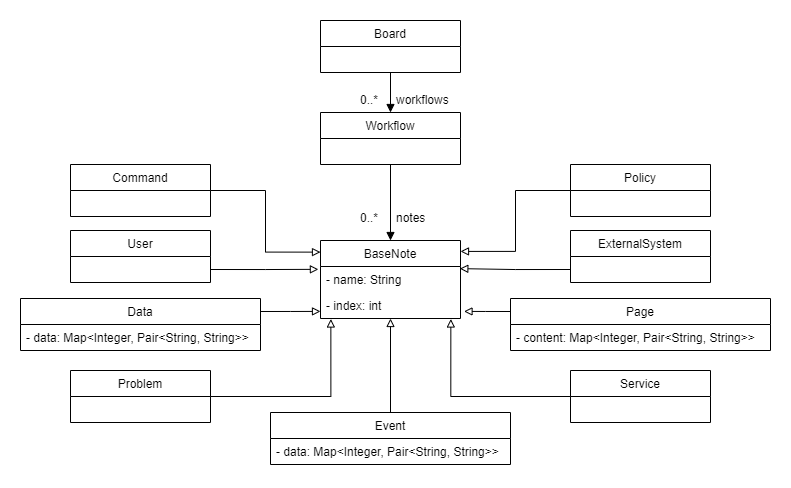
\includegraphics[width=1\textwidth]{images/3.1/classdiagram.drawio}
    \caption{Klassendiagramm fulibWorkflows}
    \label{fig:classdiagram}
\end{figure}

Bevor anhand eines Beispiels die Verwendung einer exit-Methode erläutert wird, ist es notwendig das Datenmodell genauer zu betrachten.
In Abbildung~\ref{fig:classdiagram} ist das Klassendiagramm abgebildet, welches die Struktur eines \ac{ES}-Boards nach dem Parsen der YAML-Eingabe widerspiegelt.
Jeder Note besitzt eine dazugehörige Klasse, welche von BaseNote erbt.
Für jeden Note existiert somit ein Name und ein Index, auf welchen im folgenden Abschnitt eingegangen wird.
Da es im Event Storming ein dazugehöriges \textit{Board} gibt, ist dies ebenfalls eine Klasse, welche alle \textit{workflows} einer Eingabe hält.
Ein Workflow besteht weiterhin aus vielen Notes.
Wie zuvor bereits erläutert, sind Data, Event und Page Sonderfälle unter den Notes, da diese weitere Daten beherbergen.
Daher haben diese Klassen ein Attribut, welches diese Daten organisiert in einer Map hält.
Hierbei wird als key der Index eines Notes verwendet und das value ist ein Pair.
Das Pair beinhaltet den Bezeichner und den dazugehörigen Wert einer zusätzlichen Property eines Notes.

\begin{listing}[!ht]
    \inputminted[firstnumber=106]{java}{listings/3.1.3/ExitPage.java}
    \caption{exitPage-Methode}
    \label{listing:exitpage}
\end{listing}

In Listing~\ref{listing:exitpage} wird ein neues Page-Objekt erstellt.
Bevor jedoch die exitPage-Methode aufgerufen wird, werden alle Elemente der Page in der Variable \textit{noteData} gespeichert.
Diese Elemente werden in der exitElement-Methode hinzugefügt, der Name einer Page wird hingegen in der gesonderten exitPageName-Methode zu \textit{noteData} hinzugefügt.
Zusätzlich zu den Daten eines Notes, wird diesem ein Index gegeben und anschließend zur Liste aller Notes hinzugefügt.
Der Index ist notwendig, um die Reihenfolge von Notes und deren Attributen beizubehalten.
